%\documentclass[notes,usenames,dvipsnames]{beamer}
%\documentclass[notes]{beamer}       % print frame + notes
%\documentclass[notes=only]{beamer}   % only notes
\documentclass[usenames,dvipsnames]{beamer}             % only frames
\usepackage{pgfpages}
%\setbeameroption{show notes on second screen}
%\setbeameroption{show notes}
%subfigures
\usepackage{caption}
\usepackage{subcaption}

%tables packages
\usepackage{multirow}

% math
\usepackage{amsmath}

% bash command
\usepackage{graphicx}
\usepackage{listings}
% varbatim for ascii figures
\usepackage[T1]{fontenc}
\usepackage[utf8]{inputenc}
%\usepackage{verbatim}
\usepackage{lipsum} % for context
\usepackage{fancyvrb}
\usepackage{varwidth}
\usepackage{circuitikz}
\ctikzset{logic ports=ieee}


\newsavebox{\asciigcn}

% notes prefixed in pympress
\addtobeamertemplate{note page}{}{\thispdfpagelabel{notes:\insertframenumber}}
%theme used
\usetheme{Madrid}
%Information to be included in the title page:
\title[Computer Architecture] %optional
{Computer Architecture}

\subtitle{Course no. 5 - CPU Architecture}

\author[Ștefan-Dan Ciocîrlan] % (optional, for multiple authors)
{}

\institute[NUSTPB] % (optional)
{
  \inst{}%
  National University of Science and Technology\\
  POLITEHNICA Bucharest
}

\date[NUSTPB 2025] % (optional)
{Computer Architecture}

\logo{
\includegraphics[height=0.9cm]{../../media/LOGO_UNSTPB_en.png}
\includegraphics[height=0.9cm]{../../media/logoACSQ.jpeg}
}


% Roman numerals
\newcommand*{\rom}[1]{\expandafter\@slowromancap\romannumeral #1@}
%split
\usepackage{amsmath}
%colors
%\usepackage[usenames,dvipsnames]{color} %loaded by the dcoument class
%subfigure
\usepackage{subcaption}
% block over block uncover
\setbeamercovered{invisible}
%\setbeamercovered{transparent}

%extra slide content
\AtBeginSection[]
{
  \begin{frame}
    \frametitle{Content}
    \tableofcontents[currentsection]
  \end{frame}
}
%notes or not
%\setbeamertemplate{note page}[plain]

\begin{document}

\frame{\titlepage}

\section{CPU components}
\begin{frame}
    \frametitle{Register}
    \begin{circuitikz}
        \draw
        (0,0) node[draw, minimum width=2cm, minimum height=3cm] (chip) {Register}
        (chip.west) ++(-0.5,1) node[left] {Data Input (DI)} -- (chip.west |- 0,1)
        (chip.west) ++(-0.5,0) node[left] {Write Enable (WE)} -- (chip.west |- 0,0)
        (chip.west) ++(-0.5,-1) node[left] {Output Enable (OE)} -- (chip.west |- 0,-1)
        (chip.east) ++(0.5,0) node[right] {Data Output (DO)} -- (chip.east |- 0,0);
    \end{circuitikz}
    
    \note{
    }
\end{frame}

\begin{frame}
    \frametitle{General Purpose Registers (GR)}
    \begin{table}[]
        \begin{tabular}{|l|l|l|}
            \hline
            \textbf{Register} & \textbf{Acronym} & \textbf{Size} \\ \hline
            Register A & RA & 16-bit \\ \hline
            Register B & RB & 16-bit \\ \hline
            Register C & RC & 16-bit \\ \hline
            Stack Pointer Register & SP & 16-bit \\ \hline
            Index Register A & XA & 16-bit \\ \hline
            Index Register B & XB & 16-bit \\ \hline
            Base Address A & BA & 16-bit \\ \hline
            Base Address B & BB & 16-bit \\ \hline
        \end{tabular}
    \end{table}
    \note{
    }
\end{frame}


\begin{frame}
    \frametitle{Registers File (RF)}
    
    \begin{circuitikz}
        % Demux
        \draw
        (0,0) node[muxdemux, muxdemux def={Lh=4, Rh=8, NL=3, NR=8, NT=0, NB=3, w=2,
        square pins=1}] (C) at (0,0) {I};
        % Inputs
    \node[left, font=\tiny] at (C.lpin 1) {DI};
    \node[left, font=\tiny] at (C.lpin 2) {WE};
    \node[left, font=\tiny] at (C.lpin 3) {OE};
    
    % Outputs
    \node[above, font=\tiny] at (C.rpin 1) {RA};
    \node[right, font=\tiny] at (C.rpin 2) {RB};
    \node[right, font=\tiny] at (C.rpin 3) {RC};
    \node[right, font=\tiny] at (C.rpin 4) {SP};
    \node[right, font=\tiny] at (C.rpin 5) {XA};
    \node[right, font=\tiny] at (C.rpin 6) {XB};
    \node[right, font=\tiny] at (C.rpin 7) {BA};
    \node[right, font=\tiny] at (C.rpin 8) {BB};
    \node[below, font=\tiny] at (C.bpin 1) {Register Address (REG)};
    
    % Split RA output into 3 connections
    \draw (C.rpin 1) -- ++(1.0,0) coordinate (split) 
    (split) |- ++(1,1.0) node[right, font=\tiny] {DI}
    (split) |- ++(1,-1.0) node[right, font=\tiny] {WE}
    (split) -- ++(1,0) node[right, font=\tiny] {OE};
    
    % Connect to another component
    \draw (split) -- ++(1,0) node[draw, minimum width=2cm, minimum height=3cm, anchor=west] (chip) {RA}
    (chip.east) node[left, font=\tiny] {DO}
    (chip.east) |- ++(1,0.0) node[muxdemux, muxdemux def={Lh=8, Rh=1, NL=8, NR=1, NT=0, NB=3, w=2,
    square pins=1}] (D) at (6.5,0) {O};
    % Inputs
    \node[above, font=\tiny] at (D.lpin 1) {RA};
    \node[left, font=\tiny] at (D.lpin 2) {RB};
    \node[left, font=\tiny] at (D.lpin 3) {RC};
    \node[left, font=\tiny] at (D.lpin 4) {SP};
    \node[left, font=\tiny] at (D.lpin 5) {XA};
    \node[left, font=\tiny] at (D.lpin 6) {XB};
    \node[left, font=\tiny] at (D.lpin 7) {BA};
    \node[left, font=\tiny] at (D.lpin 8) {BB};
    \node[below, font=\tiny] at (D.bpin 1) {Register Address (REG)};

    % Outputs
    \node[above, font=\tiny] at (D.rpin 1) {DO};

    \end{circuitikz}
\end{frame}

\begin{frame}
    \frametitle{Special Purpose Registers}
    \begin{table}[]
        \begin{tabular}{|l|l|l|}
            \hline
            \textbf{Register} & \textbf{Acronym} & \textbf{Size} \\ \hline
            Program Counter & PC & 16-bit \\ \hline
            Instruction Register & IR & 16-bit \\ \hline
            Memory Address Register & MA & 16-bit \\ \hline
            Flags Register & FR & 16-bit \\ \hline
            Operand Register 1 & T1 & 16-bit \\ \hline
            Operand Register 2 & T2 & 16-bit \\ \hline
            Input/Output Addressing Register & IOA & 16-bit \\ \hline
        \end{tabular}
    \end{table}
\end{frame}

\begin{frame}
    \frametitle{Memory (M)}
    \begin{itemize}
        \item Address width: 16-bit
        \item Data width: 16-bit
    \end{itemize}
    \begin{circuitikz}
        \draw
        (0,0) node[draw, minimum width=2cm, minimum height=4cm] (chip) {Memory}
        (chip.west) ++(-0.5,1) node[left] {Address (MA)} -- (chip.west |- 0,1)
        (chip.west) ++(-0.5,0.5) node[left] {Memory Input (MI)} -- (chip.west |- 0,0.5)
        (chip.west) ++(-0.5,-0.5) node[left] {Write Enable (WE)} -- (chip.west |- 0,-0.5)
        (chip.west) ++(-0.5,-1) node[left] {Output Enable (OE)} -- (chip.west |- 0,-1)
        (chip.east) ++(0.5,0) node[right] {Memory Output (MO)} -- (chip.east |- 0,0);
    \end{circuitikz}

\end{frame}

\begin{frame}
    \frametitle{Arithmetic Logic Unit (ALU)}
    \begin{circuitikz}
        \draw
        (0,0) node[muxdemux, muxdemux def={Lh=7, NL=2, Rh=4, NR=2, NB=1, NT=2, w=4,
        inset w=1, inset Lh=2, inset Rh=0, square pins=1}] (chip) {ALU}
        % Inputs
        (chip.lpin 1) node[left] {Operand 1 (T1)}
        (chip.lpin 2) node[left] {Operand 2 (T2)}
        (chip.bpin 1) node[below] {Operation (OP)}
        (chip.tpin 1) node[left] {Carry In (CI)}
        (chip.tpin 2) node[right] {Output Enable (OE)}

        % Outputs
        (chip.rpin 1) node[right] {Result (R)}
        (chip.rpin 2) node[right] {Flags (FR)};

    \end{circuitikz}
\end{frame}

\begin{frame}
    \frametitle{Internal Bus}
    \begin{table}[]
        \resizebox{\textwidth}{!}{%
        \begin{tabular}{|l|l|l|l|l|l|l|l|l|l|l|l|}
            \hline
            \textbf{Source} & \textbf{GR} & \textbf{M} & \textbf{T1} & \textbf{T2} & \textbf{IR} & \textbf{PC} & \textbf{IO} & \textbf{IOA} & \textbf{ALU} & \textbf{MA} & \textbf{FR} \\ \hline
            \textbf{GR} & X & X & X & X & - & X & X & - & - & X & - \\ \hline
            \textbf{M} & X & X & X & X & X & X & X & - & - & X & X \\ \hline
            \textbf{T1} & - & - & - & - & - & - & - & - & X & - & - \\ \hline
            \textbf{T2} & - & - & - & - & - & - & - & - & X & - & - \\ \hline
            \textbf{IR} & - & - & - & - & - & - & - & X & - & - & - \\ \hline
            \textbf{PC} & X & X & - & - & - & X & - & - & - & X & - \\ \hline
            \textbf{IO} & X & X & - & - & - & - & - & - & - & - & - \\ \hline
            \textbf{IOA} & - & - & - & - & - & - & X & - & - & - & - \\ \hline
            \textbf{ALU} & X & X & X & X & - & X & - & - & - & X & X \\ \hline
            \textbf{MA} & - & - & - & - & - & - & - & - & - & - & - \\ \hline
            \textbf{FR} & - & X & - & - & - & - & - & - & - & - & - \\ \hline
        \end{tabular}
        }
    \end{table}
    
\end{frame}

\section{Architecture} 
\begin{frame}
    \frametitle{Architecture}
    \begin{figure}
        \centering
        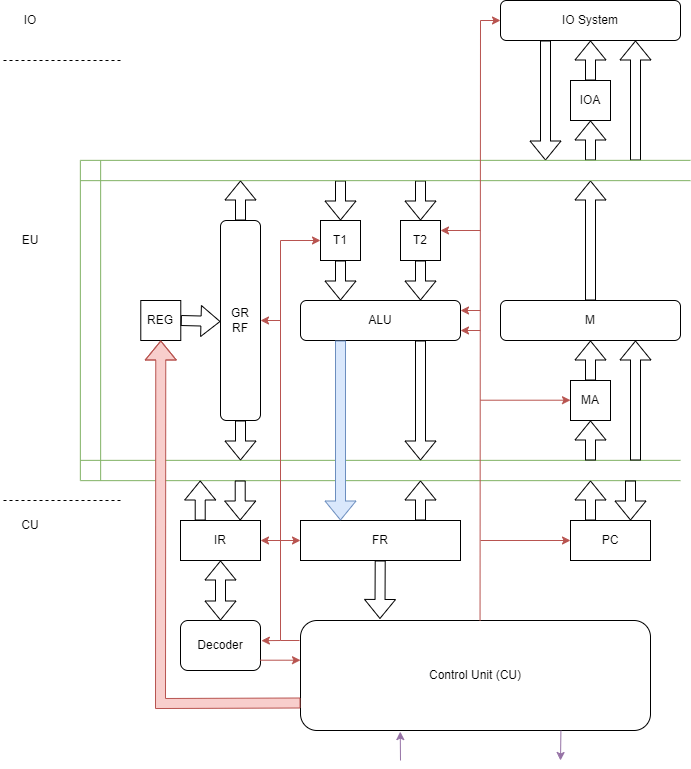
\includegraphics[height=0.7\textheight]{media/architecture.png}
        \caption{Architecture}
    \end{figure}
\end{frame}

\section{Instruction Set Architecture (ISA)}
\begin{frame}
    \frametitle{Instruction Set Architecture (ISA)}
    \textbf{Types of instructions:}
    \begin{itemize}
        \item \textbf{Data transfer}
        \item \textbf{Arithmetic}
        \item \textbf{Logical and bit manipulation}
        \item \textbf{Flow Control}
    \end{itemize}
\end{frame}

\begin{frame}
    \frametitle{Data transfer}
    \begin{table}[]
        \resizebox{\textwidth}{!}{%
            \begin{tabular}{|l|l|l|}
                \hline
                \textbf{Goal} & \textbf{Acronym} & \textbf{Description} \\ \hline
                \multirow{3}{*}{General} & MOV & Move data from source to destination \\ \cline{2-3}
                                                & PUSH & Push data onto the stack \\ \cline{2-3}
                                                & POP & Pop data from the stack \\ \hline
                \multirow{2}{*}{IO} & IN & Input data from an I/O port \\ \cline{2-3}
                                    & OUT & Output data to an I/O port \\ \hline
                \multirow{2}{*}{Flags} & PUSHF & Push flags onto the stack \\ \cline{2-3}
                                       & POPF & Pop flags from the stack \\ \hline
            \end{tabular}
        }
    \end{table}
\end{frame}

\begin{frame}
    \frametitle{Arithmetic}
    \begin{table}[]
        \resizebox{\textwidth}{!}{%
            \begin{tabular}{|l|l|l|}
                \hline
                \textbf{Goal} & \textbf{Acronym} & \textbf{Description} \\ \hline
                \multirow{3}{*}{Addition} & ADD & Add two operands \\ \cline{2-3}
                                                & ADC & Add two operands with carry \\ \cline{2-3}
                                                & INC & Increment one operand\\ \hline
                \multirow{5}{*}{Subtraction} & SUB & Subtract destination with source \\ \cline{2-3}
                                       & SBB & Subtract with borrow \\ \cline{2-3}
                                       & DEC & Decrement one operand \\ \cline{2-3}
                                        & NEG & Negate one operand (two's complement) \\ \cline{2-3}
                                        & CMP & Compare two operands \\ \hline
            \end{tabular}
        }
    \end{table}
\end{frame}

\begin{frame}
    \frametitle{Logical and bit manipulation}
    \begin{table}[]
        \resizebox{\textwidth}{!}{%
            \begin{tabular}{|l|l|l|}
                \hline
                \textbf{Goal} & \textbf{Acronym} & \textbf{Description} \\ \hline
                \multirow{3}{*}{Logic} & AND & Bitwise AND operation \\ \cline{2-3}
                                                & OR & Bitwise OR operation \\ \cline{2-3}
                                                & XOR & Bitwise XOR operation \\ \cline{2-3}
                                                & NOT & Not one operand (one's complement) \\ \cline{2-3}
                                                & TEST & Bitwise AND without result \\ \hline
                \multirow{3}{*}{Shift} & SHL/SAL & Shift left \\ \cline{2-3}
                                    & SHR & Shift right \\ \cline{2-3}
                                    & SAR & Arithmetic shift right \\ \hline
            \end{tabular}
        }
    \end{table}
\end{frame}

\begin{frame}
    \frametitle{Flow Control}
    \begin{table}[]
        \resizebox{0.6\textwidth}{!}{%
            \begin{tabular}{|l|l|l|}
                \hline
                \textbf{Goal} & \textbf{Acronym} & \textbf{Description} \\ \hline
                \multirow{3}{*}{Jump} & JMP & Jump to an address \\ \cline{2-3}
                                                & CALL & Call a subroutine \\ \cline{2-3}
                                                & RET & Return from a subroutine \\ \cline{2-3}
                                                & IRET & Return from a interuption subroutine \\ \cline{2-3}
                                                & HLT & Halt the processor \\ \hline
                \multirow{3}{*}{Conditional}    & JA & Jump above (C or Z = 0) \\ \cline{2-3}
                                                & JAE & Jump above or equal (C = 0) \\ \cline{2-3}
                                                & JB & Jump below (C) \\ \cline{2-3}
                                                & JBE & Jump below or equal (C or Z) \\ \cline{2-3}
                                                & JC & Jump if carry (C) \\ \cline{2-3}
                                                & JE & Jump if equal (Z) \\ \cline{2-3}
                                                & JG & Jump if greater ($(S \oplus O) | Z = 0$) \\ \cline{2-3}
                                                & JGE & Jump if greater or equal ($(S \oplus O) = 0$) \\ \cline{2-3}
                                                & JL & Jump if less ($(S \oplus O) = 1$) \\ \cline{2-3}
                                                & JLE & Jump if less or equal ($(S \oplus O) | Z = 1$) \\ \cline{2-3}
                                                & JNC & Jump if not carry \\ \cline{2-3}
                                                & JNE & Jump if not equal \\ \cline{2-3}
                                                & JNO & Jump if not overflow \\ \cline{2-3}
                                                & JPO & Jump if parity odd \\ \cline{2-3}
                                                & JNS & Jump if sign \\ \cline{2-3}
                                                & JO & Jump if overflow \\ \cline{2-3}
                                                & JPE & Jump if parity even \\ \cline{2-3}
                                                & JS & Jump if sign \\ \hline
            \end{tabular}
        }
    \end{table}
\end{frame}

\section{Instruction Coding}
\begin{frame}
    \frametitle{Format}
    \begin{table}[]
        \resizebox{\textwidth}{!}{%
            \begin{tabular}{|c|c|c|c|c|c|c|c|c|c|c|c|c|c|c|c|}
                \hline
                \multicolumn{16}{|c|}{Instruction Register (IR)} \\ \hline
                \textbf{0} & \textbf{1} & \textbf{2} & \textbf{3} & \textbf{4} & \textbf{5} & \textbf{6} & \textbf{7} & \textbf{8} & \textbf{9} & \textbf{10} & \textbf{11} & \textbf{12} & \textbf{13} & \textbf{14} & \textbf{15} \\ \hline
                \multicolumn{7}{|c|}{OPC} & d & \multicolumn{2}{|c|}{MOD} & \multicolumn{3}{|c|}{REG} & \multicolumn{3}{|c|}{RM} \\ \hline
                \multicolumn{16}{|c|}{immediate/data} \\ \hline
                \multicolumn{16}{|c|}{data} \\ \hline
            \end{tabular}
        }
        \begin{itemize}
            \item \textbf{OPC} - Operation code
            \item \textbf{d} - Destination (0 - RM, 1 - REG)
            \item \textbf{MOD} - Addressing mode
            \item \textbf{REG} - Register or extension for operation code
            \item \textbf{RM} - Register/Memory
        \end{itemize}
    \end{table}
\end{frame}

\begin{frame}
    \frametitle{OPC}
    \begin{itemize}
        \item $IR_{0}$ - 0 for addressing memory, 1 for addressing register
        \item $IR_{1}$ - 0 for one address, 1 for two addresses
        \item $IR_{2}$ - 0 for without immediate data, 1 for immediate data
        \item $IR_{1}=0, IR_{3}$ - 0 data transfer/flow control, 1 one operand
        \item $IR_{1}=1, IR_{3}$ - 0 without saving the result, 1 with saving the result
    \end{itemize}
\end{frame}

\begin{frame}
    \frametitle{OPC}
    \begin{table}[]
        \resizebox{0.8\textwidth}{!}{%
            \begin{tabular}{|l|l||l|l|l|l|}
                \hline
                \multirow{2}{*}{\textbf{$IR_{1}$}} & \multirow{2}{*}{\textbf{$IR_{3}$}} & \multicolumn{2}{|l|}{$IR_{0}=0$} & \multicolumn{2}{|l|}{$IR_{0}=1$} \\ \cline{3-6}
                                                  &                                      & $IR_{2}=0$ & $IR_{2}=1$ & \multicolumn{2}{|l|}{$IR_{2}=0$} \\ \hline  \hline
                \multirow{14}{*}{$0$}             & \multirow{7}{*}{$0$}                     & $000=\text{MOV}$ & $000=\text{MOV}$ & $000=\text{IN}$ &  \\ \cline{3-6}
                                                  &                                          & $001=$ & $001=$ & $001=\text{OUT}$ &  \\ \cline{3-6}
                                                  &                                          & $010=\text{PUSH}$ & $010=$ & $010=\text{PUSHF}$ &\\ \cline{3-6}
                                                  &                                          & $011=\text{POP}$ & $011=$ & $011=\text{POPF}$ &  \\ \cline{3-6}
                                                  &                                          & $100=\text{CALL}$ & $100=$ & $100=\text{RET}$ &  \\ \cline{3-6}
                                                  &                                          & $101=\text{JMP}$ & $101=$ & $101=\text{IRET}$ &  \\ \cline{3-6}
                                                  &                                          & $110=$ & $110=$ & $110=\text{HLT}$ & \\ \cline{3-6}
                                                  &                                          & $111=$ & $111=$ & $111=$ & \\ \cline{2-6}
                                                  & \multirow{7}{*}{$1$}                     & $000=\text{INC}$ & $000=$ & $0000=\text{JBE}$ & $1000=\text{JBA}$ \\ \cline{3-6}
                                                  &                                          & $001=\text{DEC}$ & $001=$ & $0001=\text{JB/JC}$ & $1001=\text{JAE/JNC}$ \\ \cline{3-6}
                                                  &                                          & $010=\text{NEG}$ & $010=$ & $0010=\text{JLE}$ & $1010=\text{JG}$ \\ \cline{3-6}
                                                  &                                          & $011=\text{NOT}$ & $011=$ & $0011=\text{JL}$ & $1011=\text{JGE}$ \\ \cline{3-6}
                                                  &                                          & $100=\text{SHL/SAL}$ & $100=$ & $0100=\text{JE/JZ}$ & $1100=\text{JNE/JNZ}$ \\ \cline{3-6}
                                                  &                                          & $101=\text{SHR}$ & $101=$ & $0101=\text{JO}$ & $1101=\text{JNO}$ \\ \cline{3-6}
                                                  &                                          & $110=\text{SAR}$ & $110=$ & $0110=\text{JS}$ & $1110=\text{JNS}$ \\ \cline{3-6}
                                                  &                                          & $111=$ & $111=$ & $0111=\text{JPE}$ & $1111=\text{JPO}$ \\ \hline

            \end{tabular}
        }
    \end{table}
    

\end{frame}


\begin{frame}
    \frametitle{OPC}
    \begin{table}[]
        \resizebox{0.6\textwidth}{!}{%
            \begin{tabular}{|l|l||l|l|l|l|}
                \hline
                \multirow{2}{*}{\textbf{$IR_{1}$}} & \multirow{2}{*}{\textbf{$IR_{3}$}} & \multicolumn{2}{|l|}{$IR_{0}=0$} & \multicolumn{2}{|l|}{$IR_{0}=1$} \\ \cline{3-6}
                                                  &                                      & $IR_{2}=0$ & $IR_{2}=1$ & \multicolumn{2}{|l|}{$IR_{2}=0$} \\ \hline  \hline
                \multirow{14}{*}{$1$}             & \multirow{7}{*}{$0$}                     & $000=$ & $000=$ &  &  \\ \cline{3-6}
                                                  &                                          & $001=$ & $001=$ &  &  \\ \cline{3-6}
                                                  &                                          & $010=\text{CMP}$ & $010=\text{CMP}$ &  &\\ \cline{3-6}
                                                  &                                          & $011=$ & $011=$ &  &  \\ \cline{3-6}
                                                  &                                          & $100=\text{TEST}$ & $100=\text{TEST}$ &  &  \\ \cline{3-6}
                                                  &                                          & $101=$ & $101=$ &  &  \\ \cline{3-6}
                                                  &                                          & $110=$ & $110=$ &  & \\ \cline{3-6}
                                                  &                                          & $111=$ & $111=$ &  & \\ \cline{2-6}
                                                  & \multirow{7}{*}{$1$}                     & $000=\text{ADD}$ & $000=\text{ADD}$ &  &  \\ \cline{3-6}
                                                  &                                          & $001=\text{ADC}$ & $001=\text{ADC}$ &  &  \\ \cline{3-6}
                                                  &                                          & $010=\text{SUB}$ & $010=\text{SUB}$ &  &  \\ \cline{3-6}
                                                  &                                          & $011=\text{SBB}$ & $011=\text{SBB}$ &  &  \\ \cline{3-6}
                                                  &                                          & $100=\text{AND}$ & $100=\text{AND}$ &  &  \\ \cline{3-6}
                                                  &                                          & $101=\text{OR}$ & $101=\text{OR}$ &  &  \\ \cline{3-6}
                                                  &                                          & $110=\text{XOR}$ & $110=\text{XOR}$ &  &  \\ \cline{3-6}
                                                  &                                          & $111=$ & $111=$ &  &  \\ \hline

            \end{tabular}
        }
    \end{table}
    

\end{frame}

\section{Memory addressing}
\begin{frame}
    \frametitle{Direct Addressing}
    \begin{itemize}
        \item Address is directly specified in the instruction (immediate)
        \item Example: \texttt{MOV RA, M[0x1234]}
        \item $MA = 0x1234$
    \end{itemize}
\end{frame}

\begin{frame}
    \frametitle{Indirect Addressing from Memory}
    \begin{itemize}
        \item Address is stored in memory 
        \item Example: \texttt{MOV RA, M[M[0x1234]]}
        \item Step 1: $MA = 0x1234$
        \item Step 2: $MA = M[0x1234]$ (indirect)
    \end{itemize}
\end{frame}

\begin{frame}
    \frametitle{Indirect Addressing from Register}
    \begin{itemize}
        \item Address is stored in a register
        \item Example: \texttt{MOV RA, M[BA]}
        \item $MA = BA$
    \end{itemize}
\end{frame}

\begin{frame}
    \frametitle{Indirect Addressing from base and index registers}
    \begin{itemize}
        \item Address is stored in the sum of two registers (base and index)
        \item Example: \texttt{MOV RA, M[BA + XA]}
        \item $MA = BA + XA$
    \end{itemize}
\end{frame}

\begin{frame}
    \frametitle{Indirect Addressing from base and index registers with increment after for index}
    \begin{itemize}
        \item Address is stored in the sum of two registers (base and index)
        \item Index register is incremented after the operation
        \item Example: \texttt{MOV RA, M[BA + XA++]}
        \item $MA = BA + XA$
    \end{itemize}
\end{frame}

\begin{frame}
    \frametitle{Indirect Addressing from base and index registers with decrement before for index}
    \begin{itemize}
        \item Address is stored in the sum of two registers (base and index)
        \item Index register is decremented before the operation
        \item Only with $XA$ register
        \item Example: \texttt{MOV RA, M[BA + XA--]}
        \item $MA = BA + XA - 1$
    \end{itemize}
\end{frame}

\begin{frame}
    \frametitle{Indirect Addressing from base and immediate}
    \begin{itemize}
        \item Address is stored in the sum of a base register and an immediate value
        \item Example: \texttt{MOV RA, M[BA + 0x1234]}
        \item $MA = BA + 0x1234$
    \end{itemize}
\end{frame}

\begin{frame}
    \frametitle{Indirect Addressing from index and immediate}
    \begin{itemize}
        \item Address is stored in the sum of a index register and an immediate value
        \item Example: \texttt{MOV RA, M[XA + 0x1234]}
        \item $MA = XA + 0x1234$
    \end{itemize}
\end{frame}

\begin{frame}
    \frametitle{Indirect Addressing from base and index with immediate}
    \begin{itemize}
        \item Address is stored in the sum of a base register, an index register and an immediate value
        \item Example: \texttt{MOV RA, M[BA + XA + 0x1234]}
        \item $MA = BA + XA + 0x1234$
    \end{itemize}
\end{frame}

\begin{frame}
    \frametitle{Immediate Addressing}
    \begin{itemize}
        \item Address is directly specified in the instruction (immediate)
        \item Example: \texttt{MOV RA, 7}
        \item $MA = PC + 1$ or $MA = PC + 2$
    \end{itemize}
\end{frame}

\begin{frame}
    \frametitle{Direct Register Addressing}
    \begin{itemize}
        \item Data is in a register specified in the instruction (RM)
        \item Example: \texttt{MOV RA, RB}
    \end{itemize}
\end{frame}

\begin{frame}
    \frametitle{Address Table for IR}
    \begin{table}[]
        \resizebox{0.9\textwidth}{!}{%
            \begin{tabular}{|l||l|l|l|l|}
                \hline
                \multirow{2}{*}{$RM=IR_{13:15}$} &  \multicolumn{4}{|l|}{$MOD=IR_{8:9}$} \\ \cline{2-5}
                                                  & $00$ & $01$ & $10$ & $11$ \\ \hline  \hline
                $000$ & $[BA+XA]$ & $[BA+XA+]$ & $[BA+XA+\text{Imm}]$ & $RA$ \\ \hline
                $001$ & $[BA+XB]$ & $[BA+XB+]$ & $[BA+XB+\text{Imm}]$ & $RB$ \\ \hline
                $010$ & $[BB+XA]$ & $[BB+XA+]$ & $[BB+XA+\text{Imm}]$ & $RC$ \\ \hline
                $011$ & $[BB+XB]$ & $[BB+XB+]$ & $[BB+XB+\text{Imm}]$ & $SP$ \\ \hline
                $100$ & $[XA]$ & $[BA+(--XA)]$ & $[XA+\text{Imm}]$ & $XA$ \\ \hline
                $101$ & $[XB]$ & $[BB+(--XA)]$ & $[XB+\text{Imm}]$ & $XB$ \\ \hline
                $110$ & $[BA]$ & $[\text{Imm}]$ & $[BA+\text{Imm}]$ & $BA$ \\ \hline
                $111$ & $[BB]$ & $[[\text{Imm}]]$ & $[BB+\text{Imm}]$ & $BB$ \\ \hline \hline

            \end{tabular}
        }
    \end{table}
\end{frame}

% \begin{frame}
%     \frametitle{Exam Question}
%     Template: Having the following registers value, main memory address and data, and the immediate value what is the value of the MA register if we use the X addressing mode?

%     Example: Having the following registers value, main memory address and data, and the immediate value of $0x1234$ what is the value of the MA register if we use the direct addressing mode?
    
%     \begin{columns}
%         \column{0.5\textwidth}
%     \begin{table}[]
%         \begin{tabular}{|l|l|}
%             \hline
%             \textbf{Register} & \textbf{Value} \\ \hline
%             BA & 0x1234 \\ \hline
%             BB & 0x5678 \\ \hline
%             XA & 0x0001 \\ \hline
%             XB & 0x0002 \\ \hline
%             RA & 0x0003 \\ \hline
%             RB & 0x0004 \\ \hline
%             RC & 0x0005 \\ \hline
%             SP & 0x0006 \\ \hline
%         \end{tabular}
%     \end{table}

%     \column{0.5\textwidth}
%     \begin{table}[]
%         \begin{tabular}{|l|l|}
%             \hline
%             \textbf{Memory Address} & \textbf{Data} \\ \hline
%             0x1234 & 0x0007 \\ \hline
%             0x5678 & 0x0008 \\ \hline
%         \end{tabular}
%     \end{table}
%     \end{columns}
% \end{frame}


% \begin{frame}
%     \frametitle{Exam Question}
%     Template: Having the memory addressing table and instruction format tables, what is the instruction conding for the X operation?

%     Example: Having the memory addressing table and instruction format tables, what is the instruction conding for the $MOV\ RA, [BA+XA+]$?
% \end{frame}


% \begin{frame}
%     \frametitle{Exam Question}
%     Template: Having the memory addressing table and instruction format tables, what is the instruction for the $IR=x$?

%     Example: Having the memory addressing table and instruction format tables, what is the instruction for the $IR=0x47AB$?
% \end{frame}


\section{Execution}
\begin{frame}
\frametitle{Execution 1}
\begin{columns}
\column{0.5\textwidth}
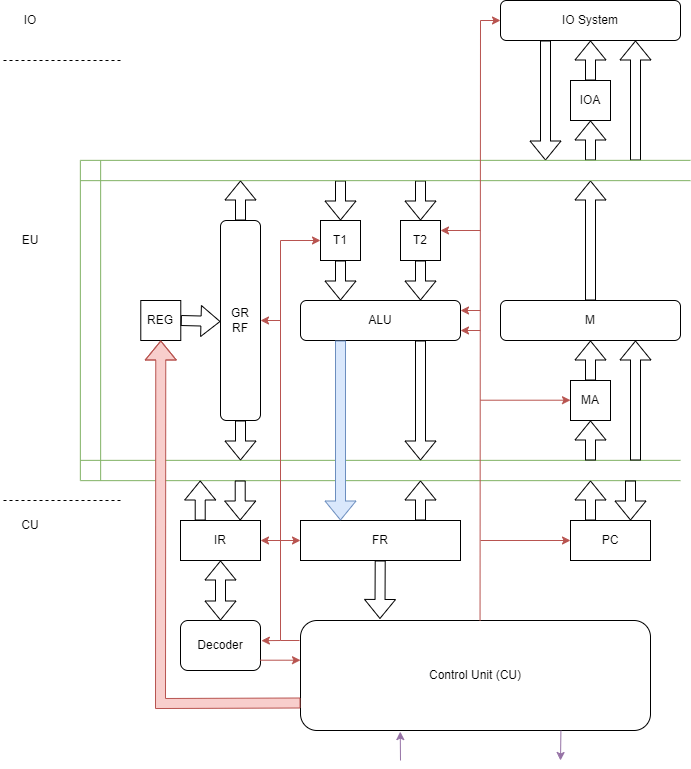
\includegraphics[width=0.9\textwidth]{media/architecture.png}
\column{0.5\textwidth}
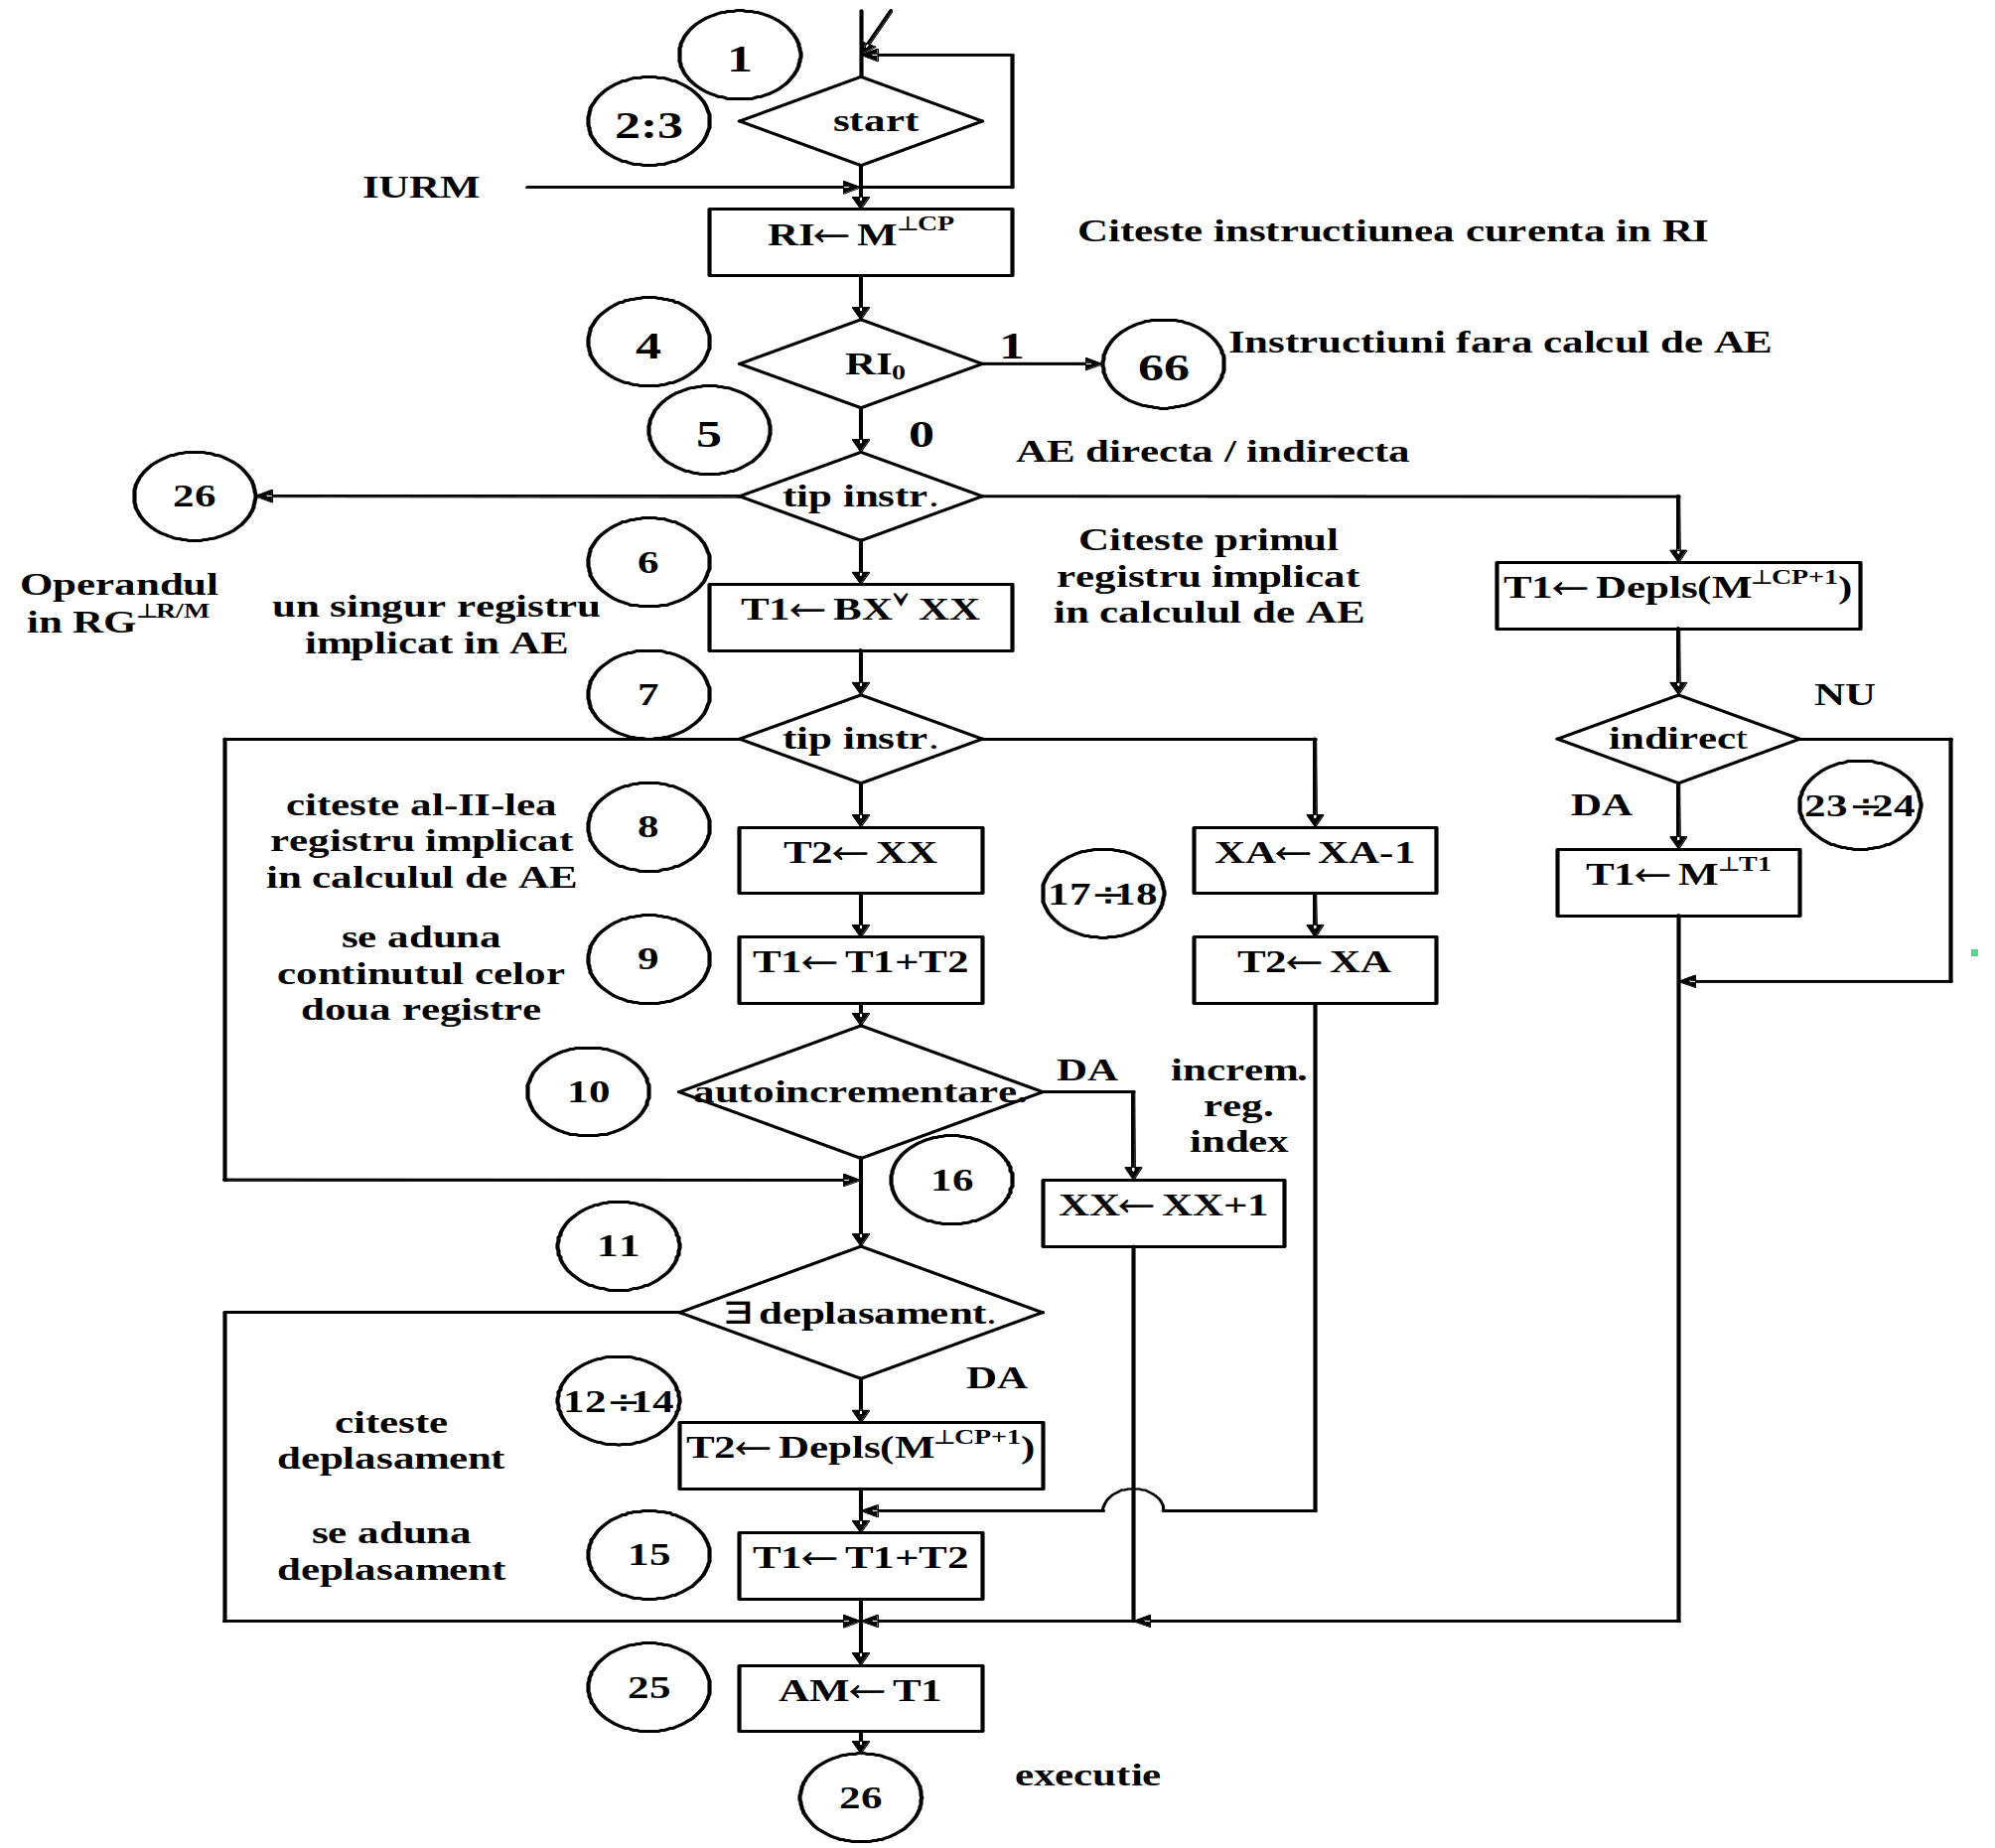
\includegraphics[width=0.9\textwidth]{media/cdtree1.png}
\end{columns}
\end{frame}

\begin{frame}
\frametitle{Execution 2}
\begin{columns}
\column{0.5\textwidth}
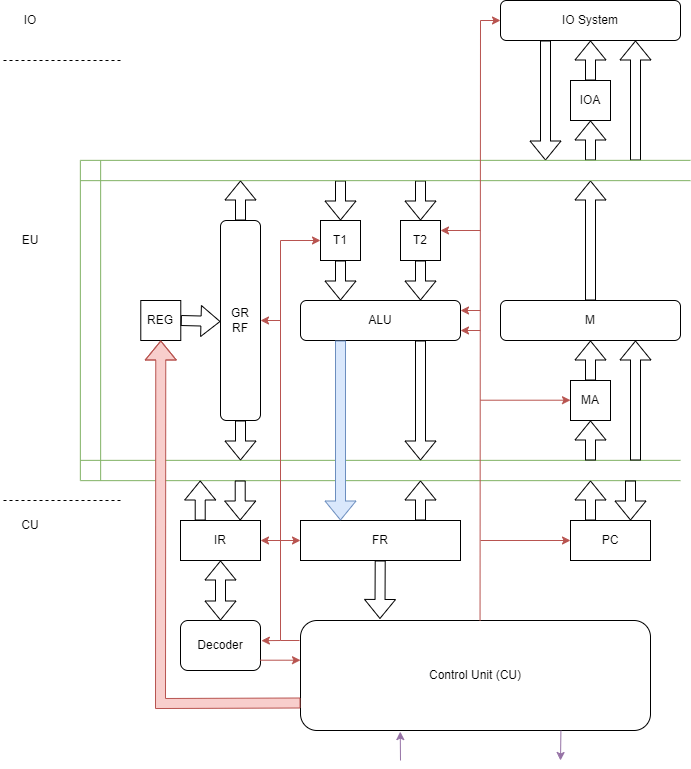
\includegraphics[width=0.9\textwidth]{media/architecture.png}
\column{0.5\textwidth}
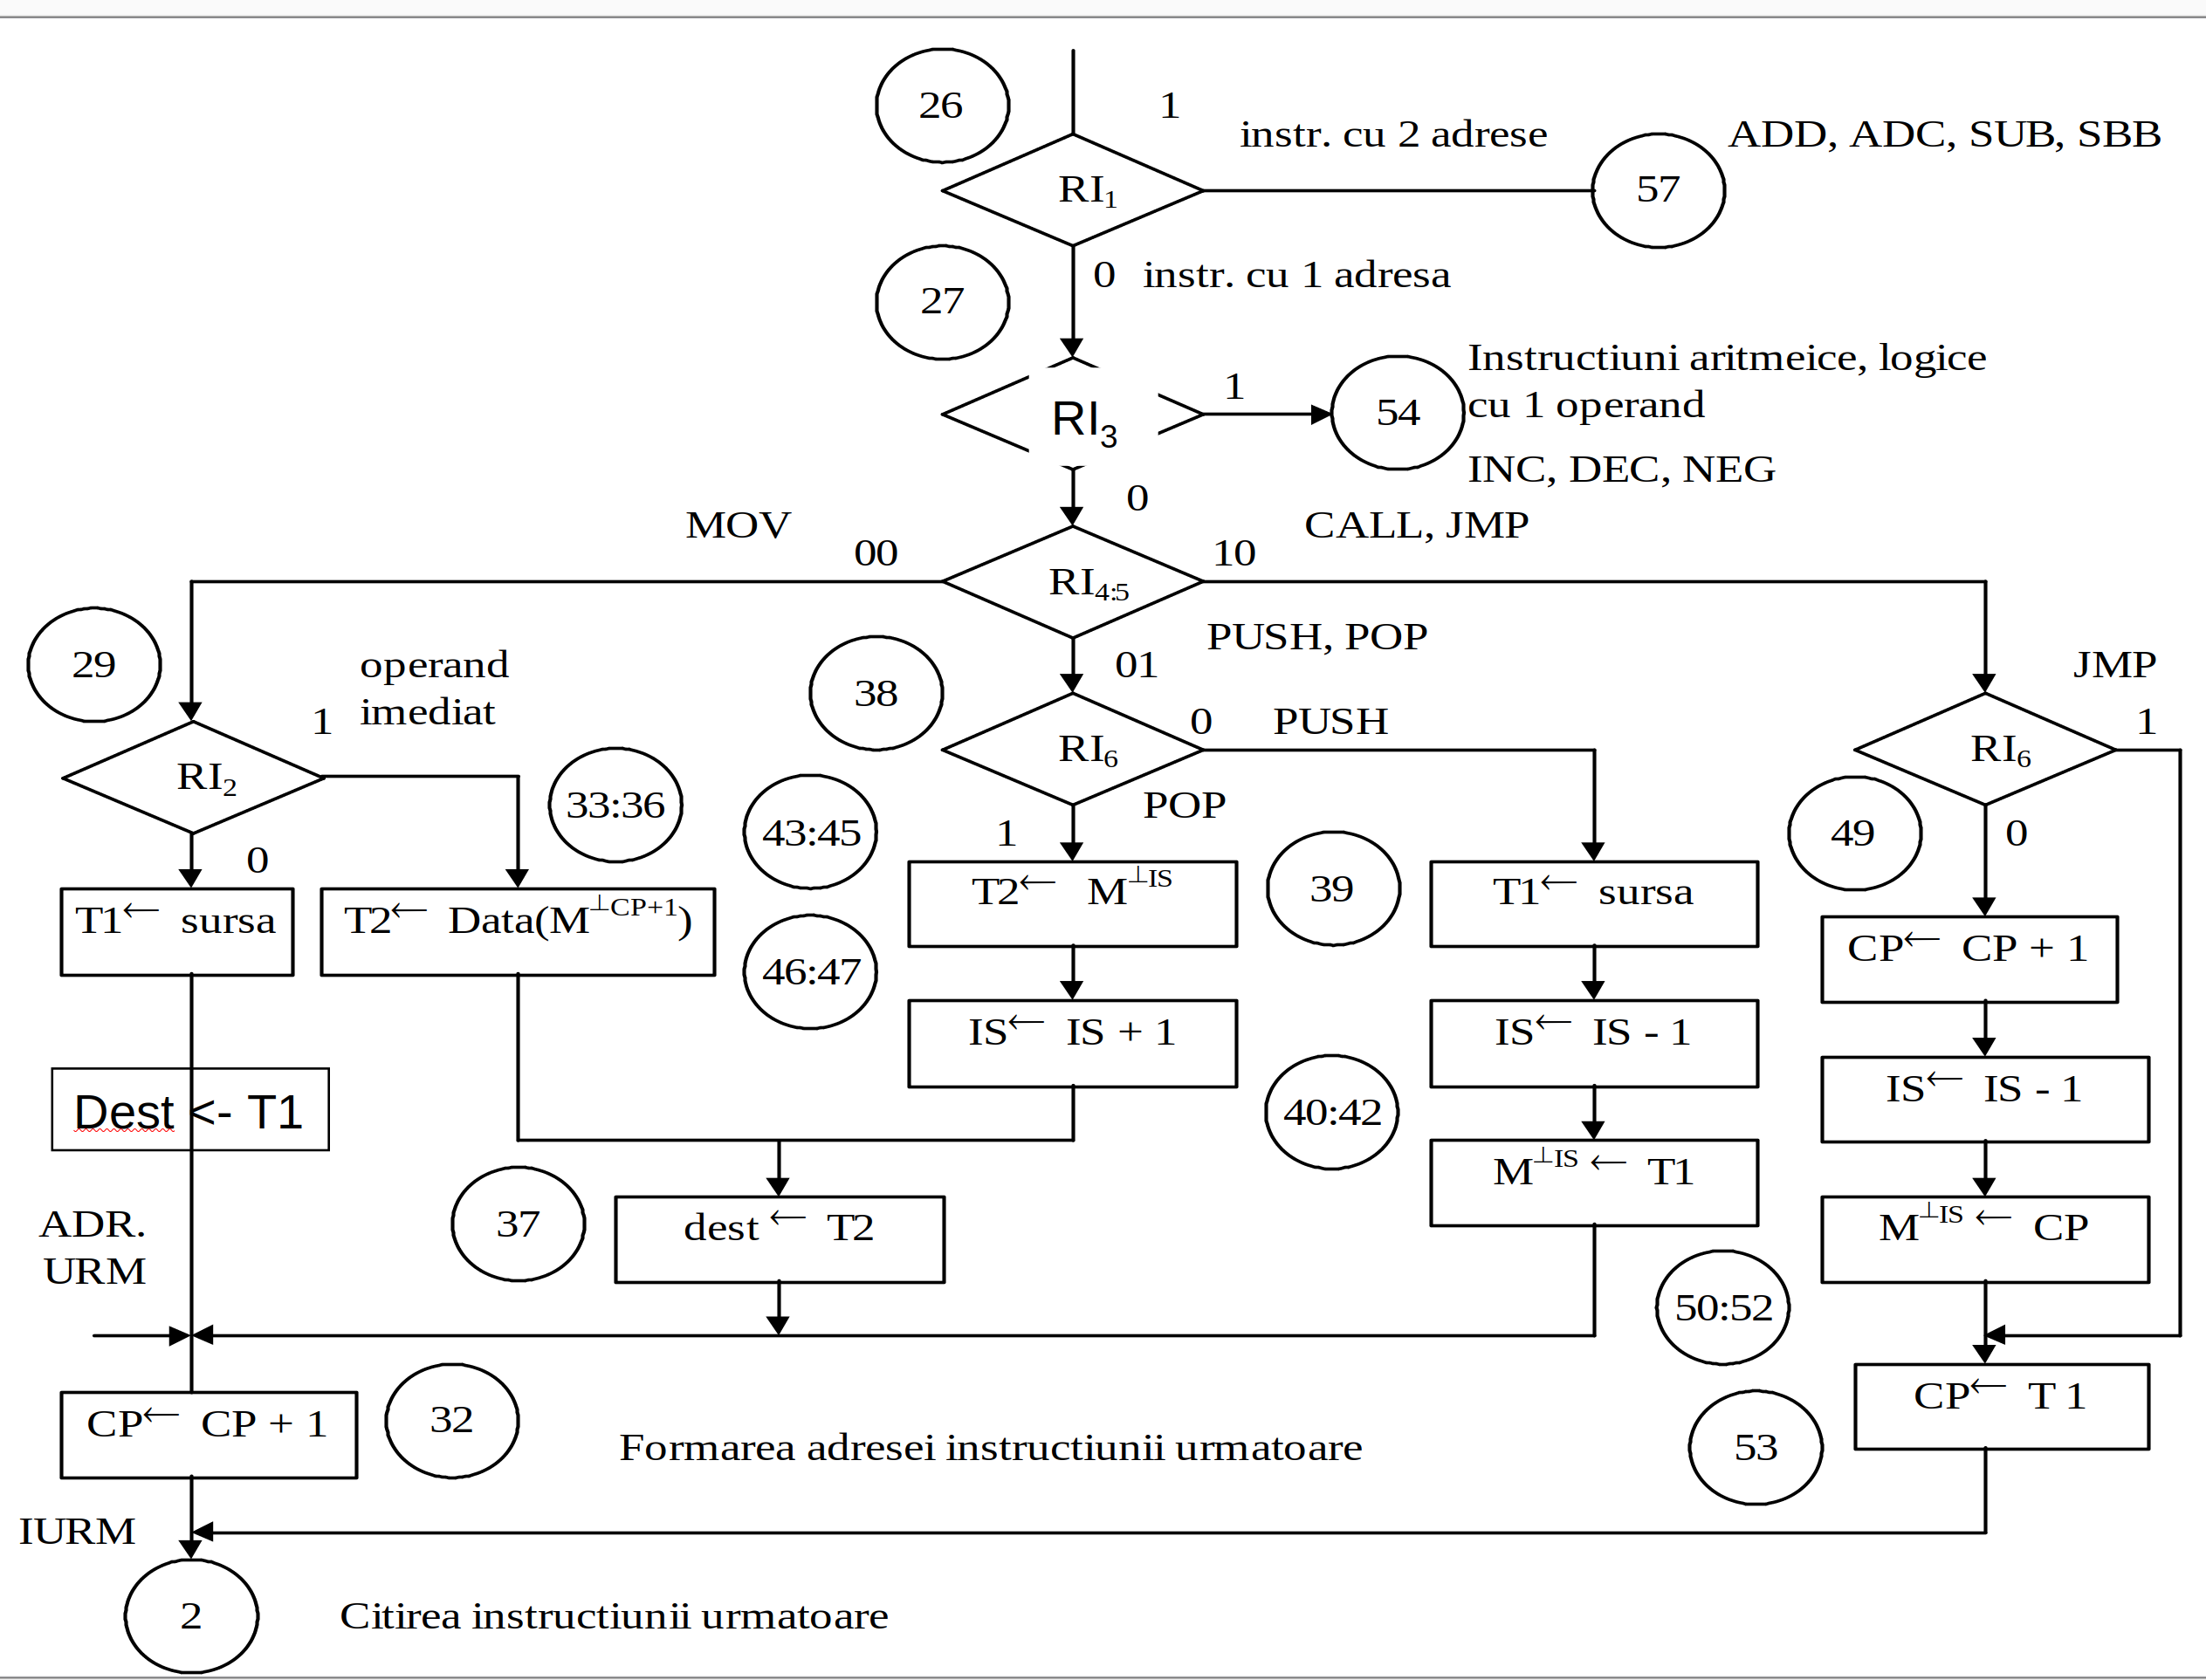
\includegraphics[width=0.9\textwidth]{media/cdtree2.png}
\end{columns}
\end{frame}



\begin{frame}
    \frametitle{Execution 3}
    \begin{columns}
    \column{0.5\textwidth}
    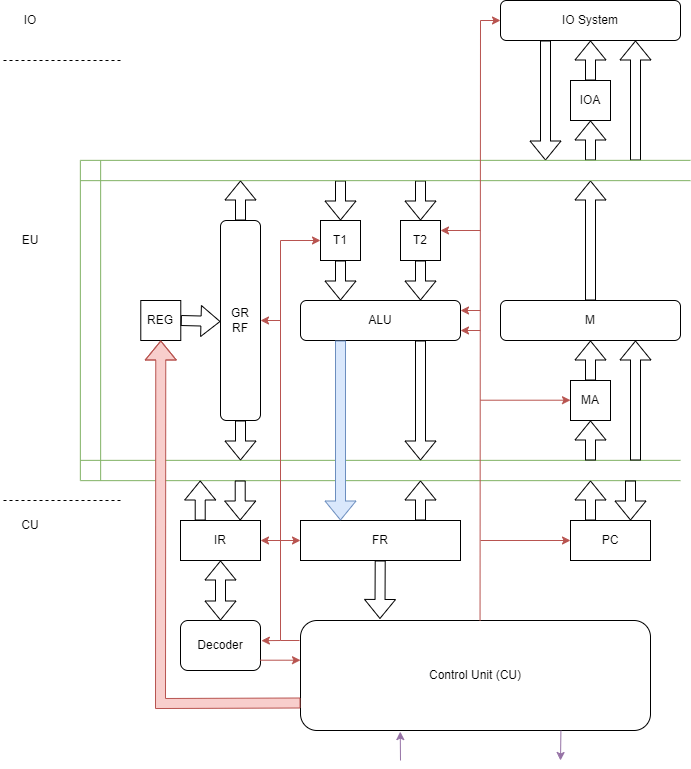
\includegraphics[width=0.9\textwidth]{media/architecture.png}
    \column{0.5\textwidth}
    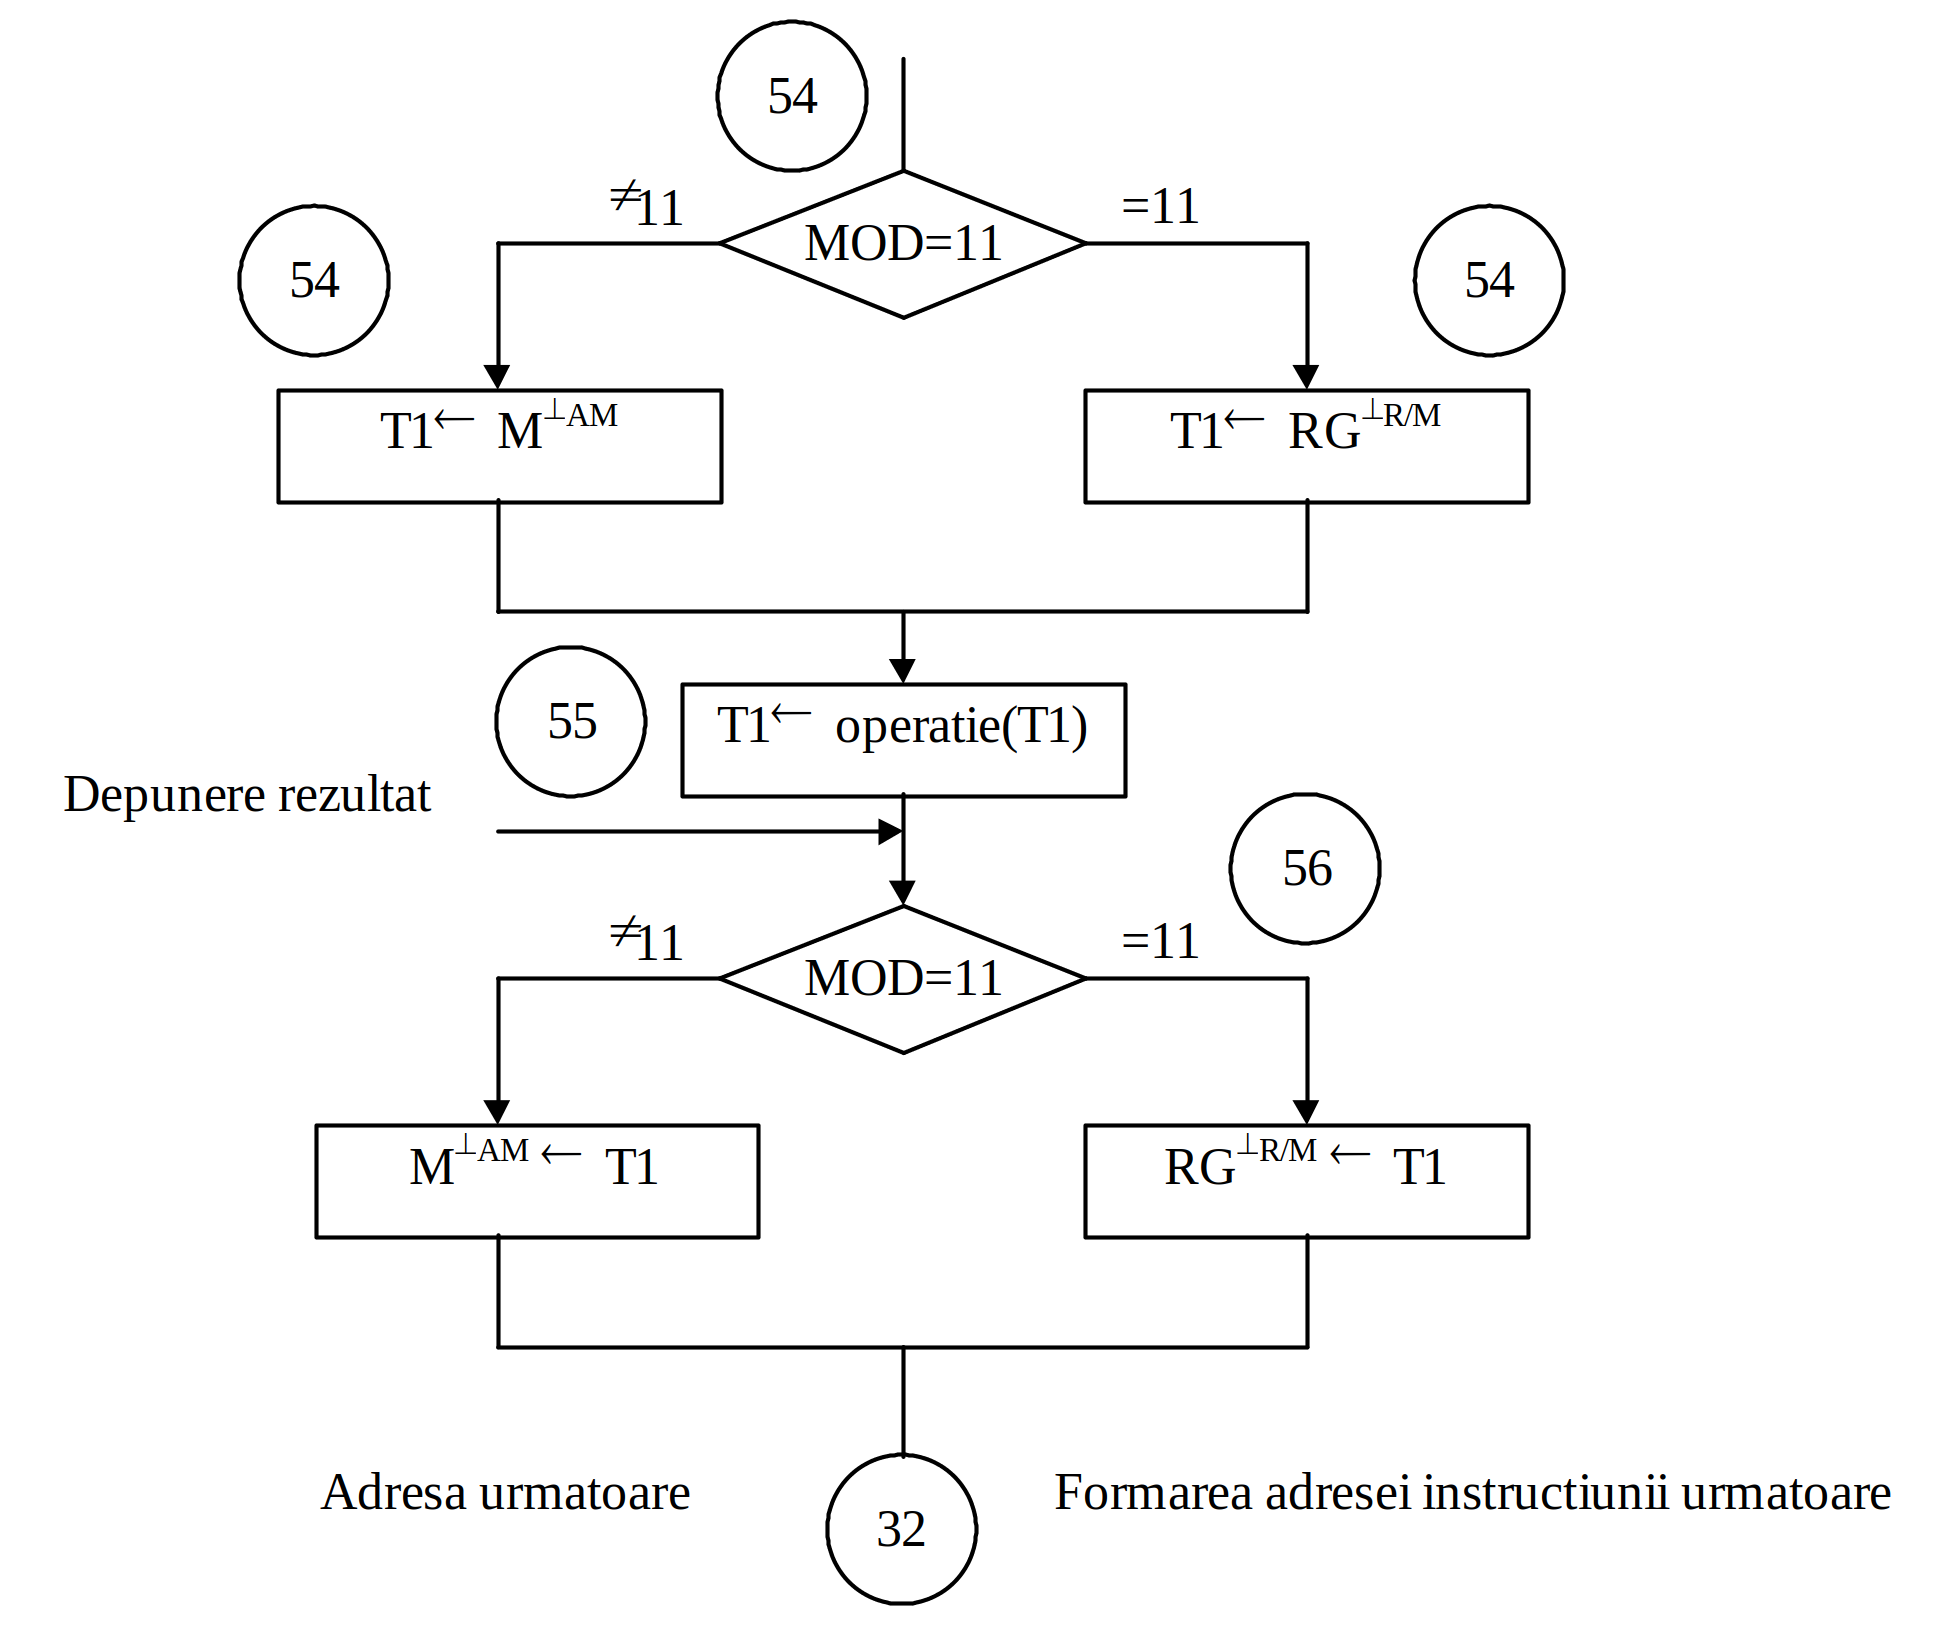
\includegraphics[width=0.9\textwidth]{media/cdtree3.png}
    \end{columns}
    \end{frame}



\begin{frame}
    \frametitle{Execution 4}
    \begin{columns}
    \column{0.5\textwidth}
    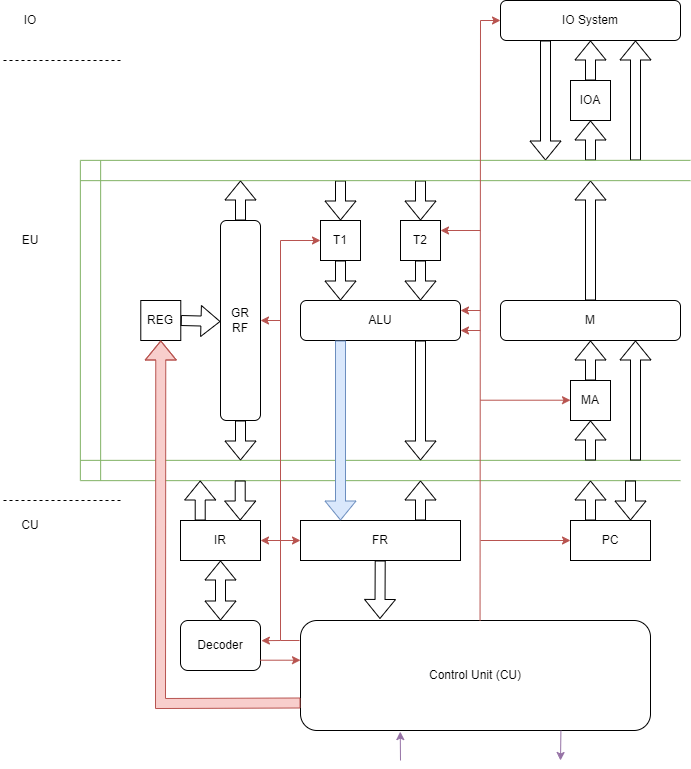
\includegraphics[width=0.9\textwidth]{media/architecture.png}
    \column{0.5\textwidth}
    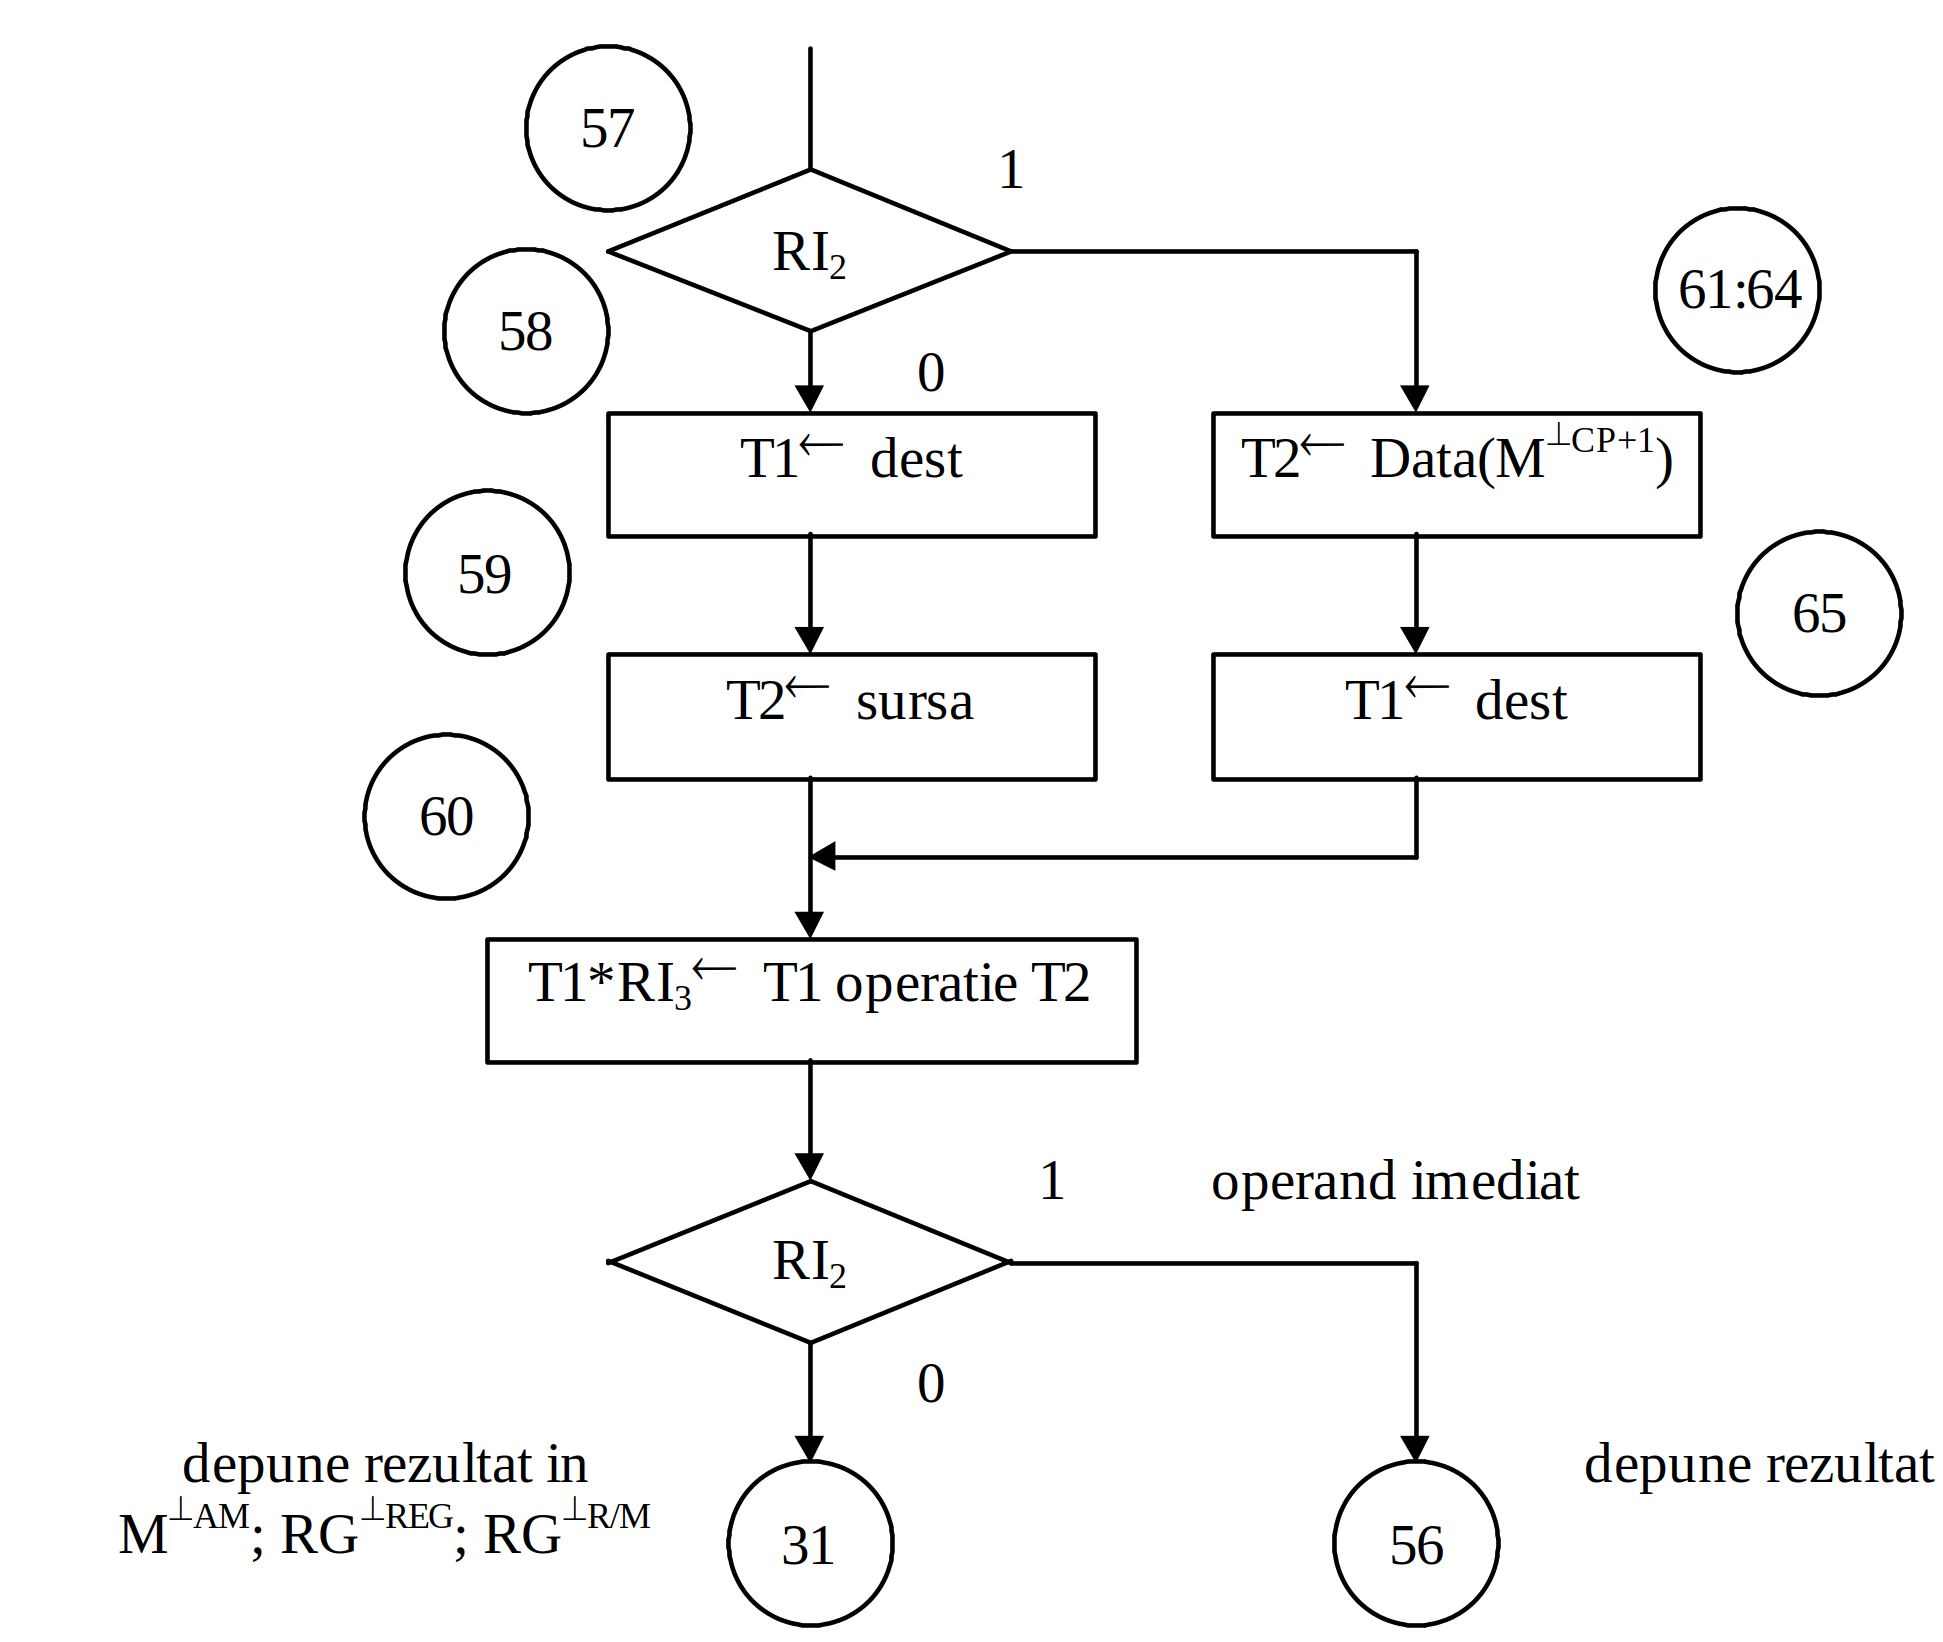
\includegraphics[width=0.9\textwidth]{media/cdtree4.png}
    \end{columns}
    \end{frame}




\begin{frame}
    \frametitle{Execution 5}
    \begin{columns}
    \column{0.5\textwidth}
    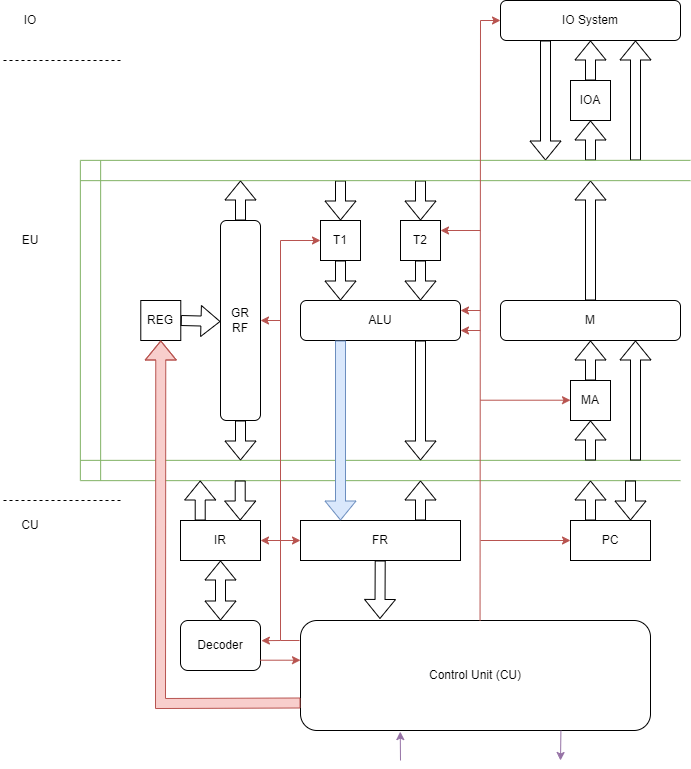
\includegraphics[width=0.9\textwidth]{media/architecture.png}
    \column{0.5\textwidth}
    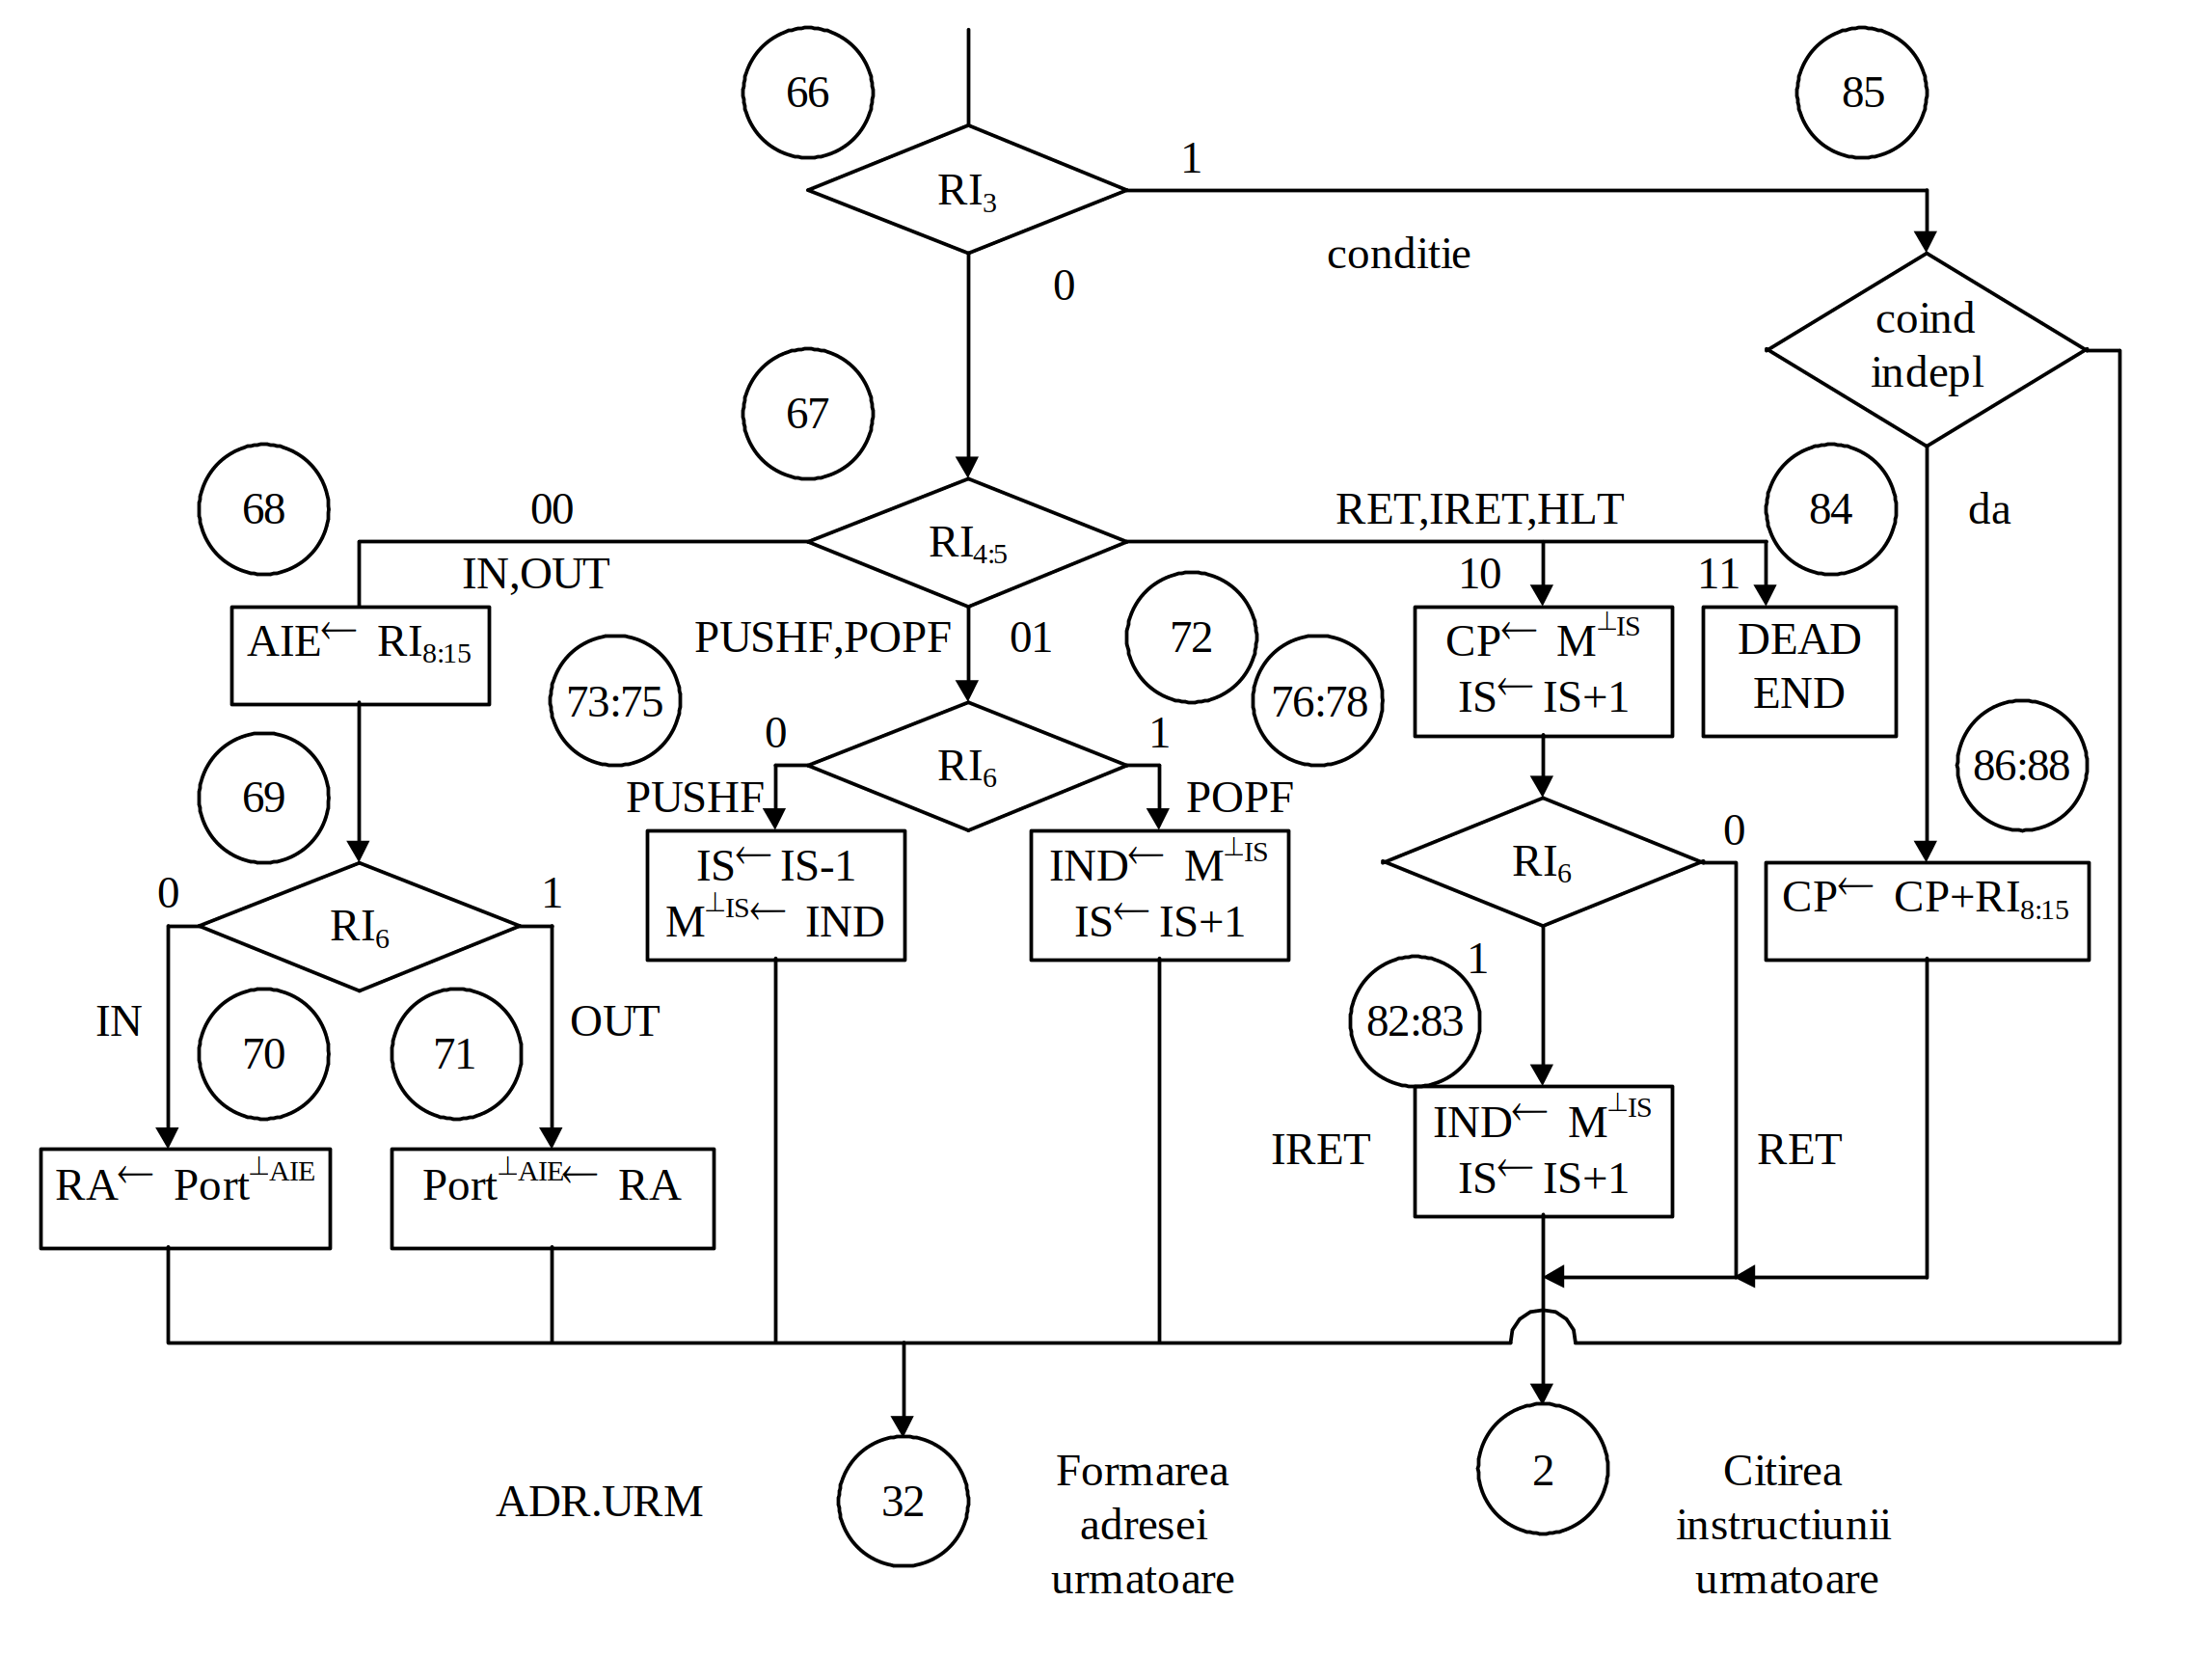
\includegraphics[width=0.9\textwidth]{media/cdtree5.png}
    \end{columns}
    \end{frame}



\section{Q\&A}
\begin{frame}
\end{frame}

%\begin{frame}
%\frametitle{Table of Contents}
%\tableofcontents
%\end{frame}


\end{document}